\documentclass[twocolumn,11pt]{sotsuken_abst}

%% 体裁
% ページレイアウト(A4:297 mm × 210 mm,1 インチ = 25.4 mm)
% http://www.biwako.shiga-u.ac.jp/sensei/kumazawa/tex/layout.html
% http://www.slis.tsukuba.ac.jp/~fujisawa.makoto.fu/cgi-bin/wiki/index.php?TeX%A5%E1%A5%E2#p61e1b46
% 上 20 mm,下 22 mm,左右 20 mm の余白設定
\setlength{\topmargin}{-20truemm}
\setlength{\headheight}{10truemm}
\setlength{\headsep}{4.6truemm}
\setlength{\textheight}{255truemm}
\setlength{\oddsidemargin}{-5.4truemm}
\setlength{\evensidemargin}{-5.4truemm}  % twoside オプション指定時のみ有効
\setlength{\textwidth}{170truemm}
% \setlength{\columnsep}{8truemm}
\setlength{\columnsep}{6truemm}

%タイトル
\title{ジャイロセンサを用いたロボットの方向自動修正}
\author{平元隆顕・松村隆平(指導教員 伊藤恒平)}
\date{2017-1-6}
\setcounter{page}{7}
\lhead{}
\chead{}
\rhead{{\sf 16・204}\\{\bf 機械工学科}}
\lfoot{}
\cfoot{{\sf-\ M-0\thepage \ -}}
%\rfoot{}
\renewcommand{\headrulewidth}{3pt}
%\renewcommand{\footrulewidth}{1pt}

\begin{document}
%\layout
\maketitle
\thispagestyle{fancy}
\pagestyle{fancy}

%行間
\setlength{\baselineskip}{5.6truemm}

%文字間
\kanjiskip=.07zw plus 3pt minus 3pt
\xkanjiskip=.07zw plus 3pt minus 3pt

%本文

\section{はじめに}

	\subsection{研究の背景}
	2016年度に行われたNHK高専ロボコン「ロボット・ニューフロンティア」に参加。内容は港町から海を渡り、新大陸へと目指すというものである。

	\subsection{研究の目的}
	今回のロボコン競技では積込みロボットの移動手段として、全方向移動可能なメカナムホイールを使用している。これにジャイロセンサを加えることで、ずれを修正しながら継続的に直進させる。

\section{メカナムホイールを採用した理由}
	出題された多くの課題をこなす為には3分という制限時間は非常に短く、丘に箱を積み上げるだけでも困難になる。そのため、メカナムホイールを使用することで二輪駆動よりも圧倒的速くに課題をクリアすることができる。

\section{メカナムホイールの説明}

	\subsection{メカナムホイールについて}
	メカナムホイールとは車輪の円周面に回転軸から図\ref{角度}のように45度傾いた樽状のタイヤを一定の間隔を空けながら覆うようにして取り付けた外見をしている。メカナムホイールには順方向に傾いた車輪と逆方向に傾いた車輪の二種類があり、図\ref{角度}を順方向とする。これらを左右で2輪ずつの計4輪を図\ref{対角}のように取り付けることで正常に動作する。

	\begin{figure}[htp]
		\begin{center}
			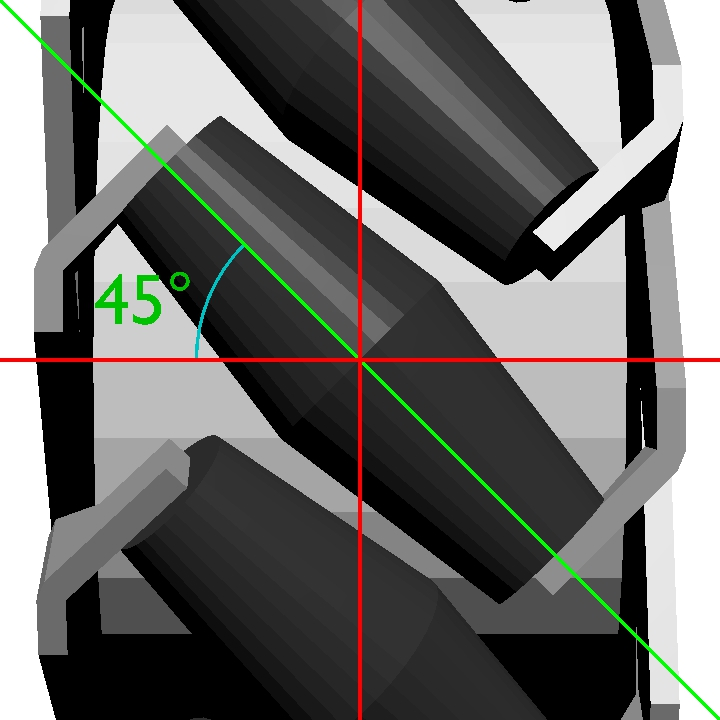
\includegraphics[width=40mm]{Image/角度.jpg}
			\caption{タイヤの角度}
			\label{角度}
		\end{center}
	\end{figure}

	\begin{figure}[htp]
		\begin{center}
			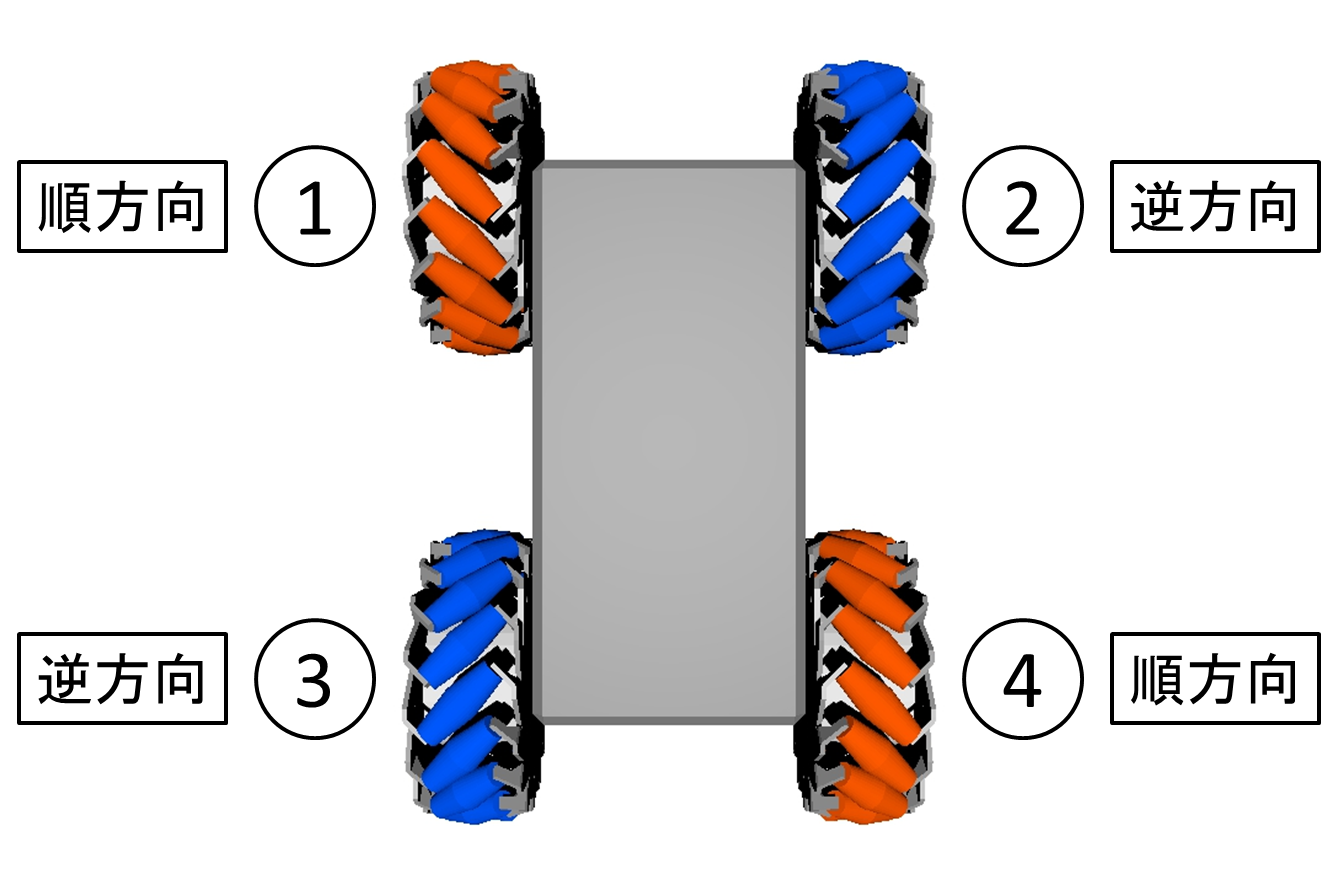
\includegraphics[width=60mm]{Image/対角.png}
			\caption{組み合わせ}
			\label{対角}
		\end{center}
	\end{figure}

	\subsection{各動作}
	単体での動作は図\ref{回転系}のように無回転と回転時ともに斜め方向にしか移動できない。次に四輪の状態での動作は車輪の回転によって発生するX方向もしくはY方向のベクトルを互いに打ち消し合うことで、図\ref{移動系}に示すように任意の方向に並行移動することができる。

	\begin{figure}[htb]
		\begin{center}
			\begin{tabular}{c}
				\begin{minipage}{0.5\hsize}
					\begin{center}
						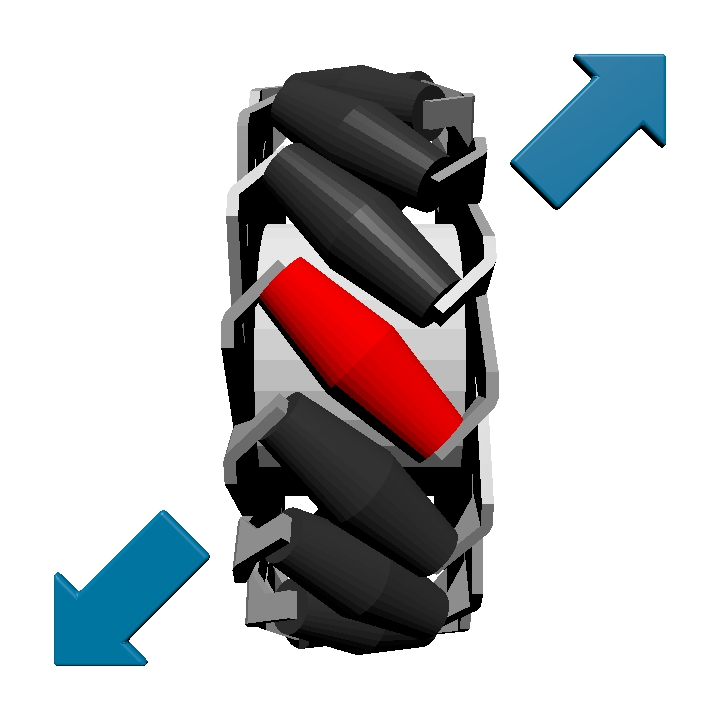
\includegraphics[width=40mm]{Image/無回転.jpg}
						\\(a)無回転
					\end{center}
				\end{minipage}
				\begin{minipage}{0.5\hsize}
					\begin{center}
						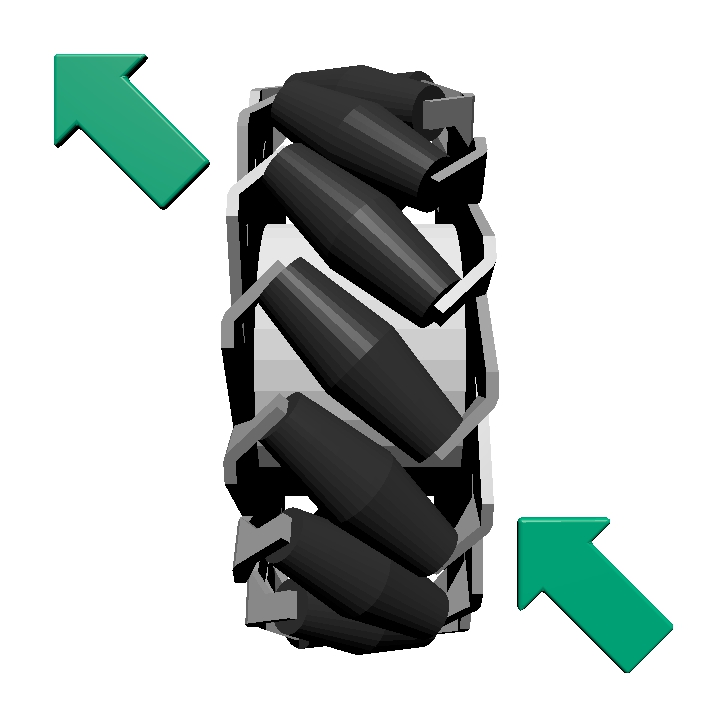
\includegraphics[width=40mm]{Image/回転.jpg}
						\\(b)回転
					\end{center}
				\end{minipage}
			\end{tabular}
			\caption{地面から見た車輪の動き}
			\label{回転系}
		\end{center}
	\end{figure}

	\begin{figure}[htb]
		\begin{center}
			\begin{tabular}{c}
				\begin{minipage}{0.33\hsize}
					\begin{center}
						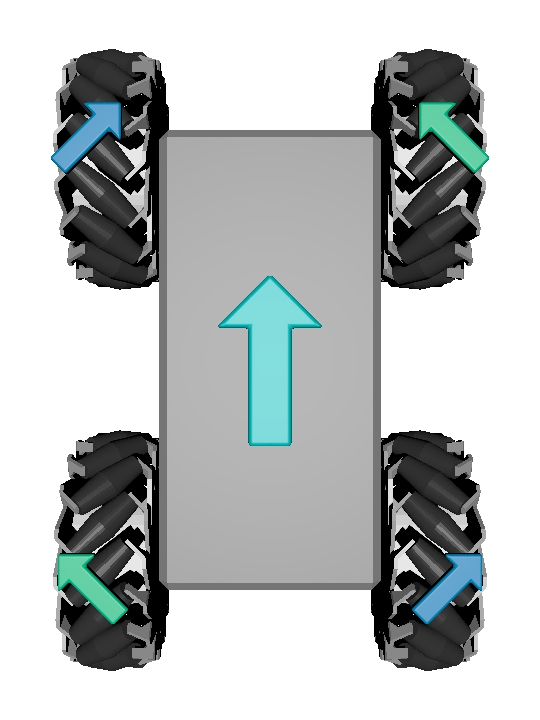
\includegraphics[width=25mm]{Image/ロボット1.jpg}
						\\(a)前進
					\end{center}
				\end{minipage}
				\begin{minipage}{0.33\hsize}
					\begin{center}
						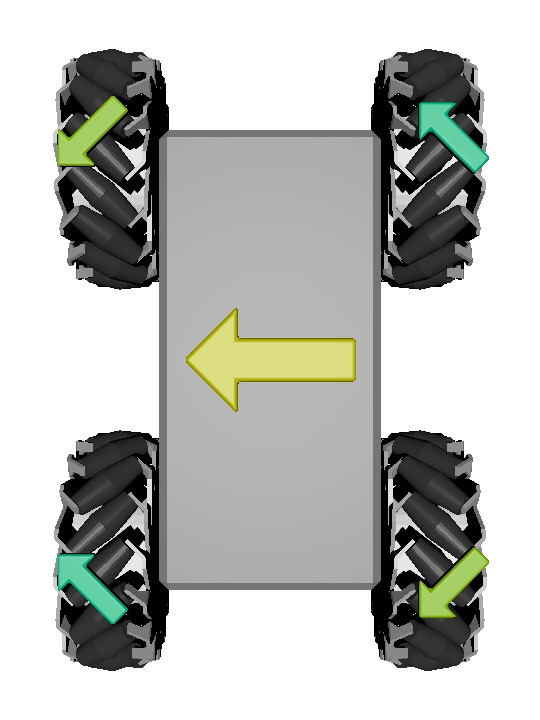
\includegraphics[width=25mm]{Image/ロボット3.jpg}
						\\(b)左並進
					\end{center}
				\end{minipage}
				\begin{minipage}{0.33\hsize}
					\begin{center}
						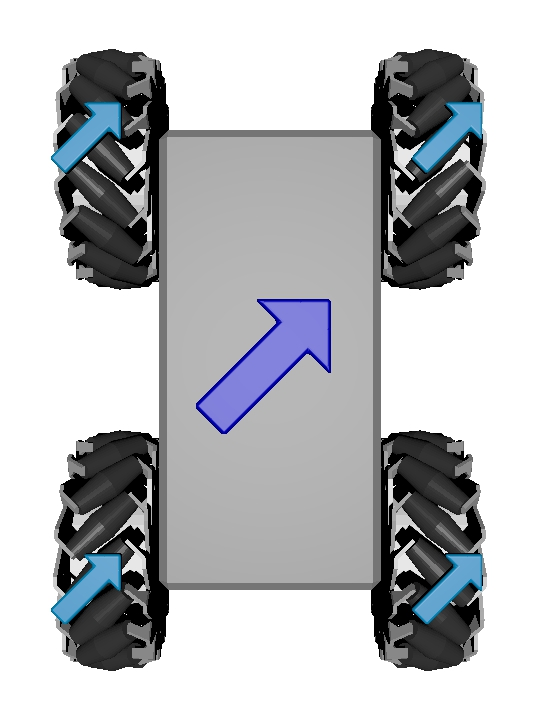
\includegraphics[width=25mm]{Image/ロボット6.jpg}
						\\(c)右斜め移動
					\end{center}
				\end{minipage}
			\end{tabular}
			\caption{真上から見たロボットの動き}
			\label{移動系}
		\end{center}
	\end{figure}

	\subsection{操作プログラム}
	メカナムホイールを操作するためには縦方向、横方向、回転方向の3種類の値が必要である。そのためDualShock3の左右のアナログスティックを用いてモータの制御を行う。アナログスティックの初期位置を原点とし、X軸とY軸の値の範囲は$-230~230$とする。左スティックは移動用で、Y方向に傾けることで$L_y$、X方向に傾けることで$L_x$を出力する。右スティックは旋回用で、X方向に傾けることで$R_x$を出力する。図\ref{対角}の番号をメカナムホイールに取り付けられたモータの番号とすると、PWM値の計算式は以下のようになる。

	\begin{eqnarray}
	M_1 = L_y + L_x + R_x
	\label{式1}
	\\
	M_2 = L_y - L_x + R_x
	\label{式2}
	\\
	M_3 = L_y - L_x + R_x
	\label{式3}
	\\
	M_4 = L_y + L_x + R_x
	\label{式4}
	\end{eqnarray}

\section{今回製作したメカナムロボの問題点}
今回製作した積込みロボットのメカナムホイールは直進中に進行方向がわずかに傾く問題が発生した。ロボットの重心が主な原因で図\ref{積込みロボット重心}に示すように重心の位置が右前に傾いている。これにより左後ろのタイヤが浮き、4輪全体が均等に力を床に伝えきれないことが問題である。

\begin{figure}[htp]
	\begin{center}
		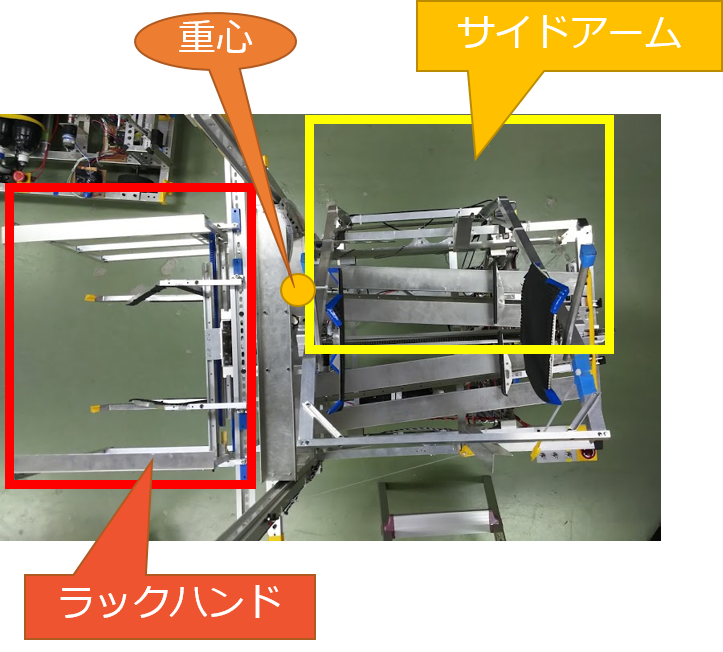
\includegraphics[width=50mm]{Image/積込みロボット重心.png}
		\caption{積込みロボット重心}
		\label{積込みロボット重心}
	\end{center}
\end{figure}

\section{方向自動修正}
図\ref{Arduino9軸モーションシールド図}のArduino9軸モーションシールドに搭載されているジャイロセンサを使用し、進行中常に正面を向けるようにする。ジャイロセンサとは、角速度センサとも呼ばれ、角度が単位時間当たりにどれだけ変化しているのか計測できるセンサである。
今回使用したプログラムでは$‐180~180[deg]$の角度を読み取ることが可能で$0[deg]$からずれた分を補正値のPWM値として式\ref{式1},\ref{式2},\ref{式3},\ref{式4}にerrの形で代入し以下のような式となる。

\begin{eqnarray}
M_1 = L_y + L_x + R_x + err
\\
M_2 = L_y - L_x + R_x + err
\\
M_3 = L_y - L_x + R_x + err
\\
M_4 = L_y + L_x + R_x + err
\end{eqnarray}

このようにすることでDualshock3の左スティックを入力中も旋回の動作が自動で行われて自動方向修正が可能となる。


\begin{figure}[htp]
	\begin{center}
		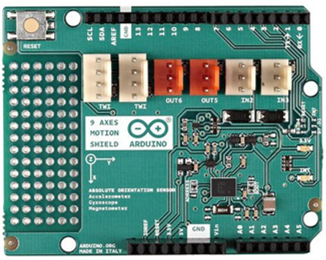
\includegraphics[width=40mm]{Image/Arduino9軸モーションシールド図.png}
		\caption{Arduino9軸モーションシールド図}
		\label{Arduino9軸モーションシールド図}
	\end{center}
\end{figure}

\section{おわりに}
メカナムホイールを用いることで容易にかつ素早く移動することができるが、ロボットの重心が中心から離れている場合、正しく移動することができない。それを改善するためには原因を修正するか、ジャイロセンサなどで補正する必要がある。

% 参考文献
\begin{thebibliography}{1}
\bibitem{gyro} Arduino9AxesMotionLibrary,http:{\slash}{\slash}www.arduino.org{\slash}learning{\slash}reference{\slash}9-axes-motion,2017{\slash}01{\slash}16閲覧
\end{thebibliography}

%%%%%%%%%%%%%%%%%%%%%%%%%%%%%%%%%%%%%%%%%%%%%%%%%%%%%%%%%%%%%%%%
\end{document}
